\chapter{INTRODUÇÃO} \label{cap:intro}
\vspace{-2cm}

A descoberta da fissão nuclear representou um importante marco na história da civilização humana. O processo, que consiste em dividir um núcleo atômico considerado instável em dois núcleos menores - pelo bombardeamento por partículas como nêutrons - é uma reação química exotérmica com grande liberação de energia. Essa descoberta proporcionou a criação de usinas nucleares para geração de energia elétrica e armas nucleares. 

Em face do potencial destrutivo das armas nucleares, mas também do enorme potencial da energia nuclear, houve a necessidade de assegurar que essa nova tecnologia fosse implementada para fins pacíficos e seguros. Com tal propósito, surgem as ferramentas de monitoramento do uso de combustíveis nucleares, que são de interesse direto de organizações internacionais, como a AIEA (Agência Internacional de Energia Atômica) e a ONU (Organização das Nações Unidas), pois podem contribuir experimentalmente em pautas relacionadas à salvaguarda de material nuclear e do desarmamento nuclear.

Uma dessas ferramentas são os detectores de antineutrinos do tipo Cherenkov. A radiação de Cherenkov consiste na radiação eletromagnética de coloração azul, ocorre quando partículas carregadas eletricamente atravessam um meio a uma velocidade superior à da luz \cite{leo2012techniques}. Nas usinas nucleares, algumas das parículas liberadas são os antineutrinos, resultantes do decaimento beta de nuclídeos gerados durante a fissão. Os detectores do tipo Cherenkov medem a radiação UV da luz gerada pelo fenômeno e, assim, estima o número de partículas que atravessaram o meio. Portanto, o uso de combustível nuclear pode ser monitorado através da relação entre a energia gerada e o número de antineutrinos detectados pelo instrumento.


\begin{figure}[H]
	\centering
		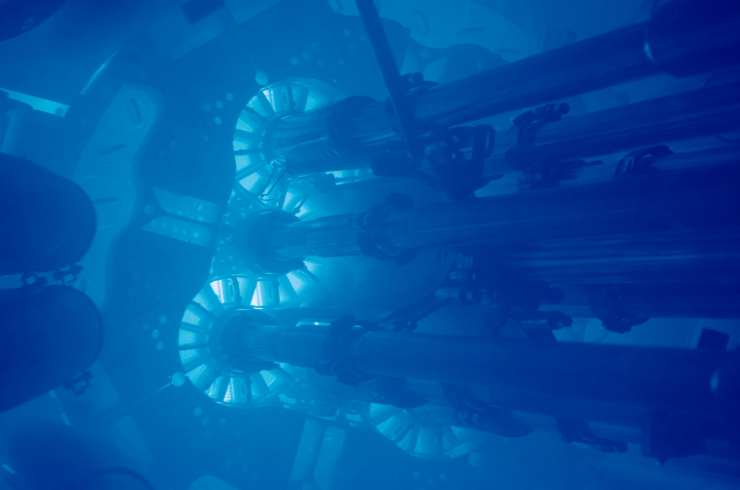
\includegraphics[width=7.7cm]{textuais/introducao/figuras/Cherenkov1.jpg}
		\caption{Radiação de Cherenkov vista em um reator nuclear}
		\label{fig:cherenkov}
\end{figure}%

No Brasil, tem-se estudado formas relativamente diferentes de aplicação  desses detectores. O experimento Neutrinos-Angra (ν-Angra), motivador do presente trabalho, é um exemplo disso. Ele foi criado com o intuito de medir a atividade de reatores nucleares, através de um detector do tipo Cherenkov, pela relação entre a  potência térmica dissipada e a taxa de eventos de antineutrinos registrados pelo detector. Um dos principais objetivos do experimento é inferir a quantidade de combustível nuclear utilizado no processo de geração de energia de maneira indireta, não invasiva e totalmente independente do sistema de controle e monitoramento do reator. 

O detector proposto pela colaboração $\nu$-Angra se baseia em um detector de superfície e, por esta razão, espera-se um ruído de fundo muito grande gerado por partículas cósmicas. Devido a este ruído, simulações da interação do detector com partículas cósmicas são importantes para melhorar a análise do sistema de diferenciação entre um evento de antineutrinos, advindo do consumo de material nuclear, e um evento de raios cósmicos.
O escopo deste trabalho é comparar os dados gerados pela simulação com o dados reais com o objetivo de medir as diferenças entre ambos os conjuntos de dados, entendendo-os e, se possível,  propondo correções no pacote de simulação.



%
%A salvaguarda de material nuclear 
%
%O experimento Neutrinos-Angra ($\nu$-Angra) foi criado com o intuito de medir a atividade de reatores nucleares através de um detector de neutrinos do tipo Cherenkov pela relação entre potência térmica dissipada e taxa de eventos de neutrinos registrados pelo detector. Um dos principais objetivos do experimento é inferir a quantidade de combustível nuclear utilizado no processo de geração de energia de maneira indireta, não invasiva e totalmente independente do sistema de controle e monitoramento do reator. Ferramentas deste tipo são de interesse direto de organizações internacionais, como a IAEA e a ONU, pois podem contribuir experimentalmente em pautas relacionadas à salvaguarda de material nuclear e desarmamento nuclear. (Carr, Rachel, et al. "Neutrino physics for Korean diplomacy." Science 362.6415 (2018): 649-650)
%
%O detector proposto pela colaboração $\nu$-Angra se baseia em um detector de superfície e, por esta razão, espera-se um ruído de fundo muito grande gerado por partículas cósmicas. Devido à este ruído, simulações da interação do detector com partículas cósmicas são importantes para melhorar a análise do sistema de diferenciação entre um evento de antineutrinos ($bar{\nu}$) advindo do consumo de material nuclear, e um evento de raios cósmicos, como múons ($\mu$). 
%
%O escopo deste trabalho é calibrar os parâmetros da simulação aos de uma aquisição de dados reais possibilitando um trufo para eventos futuros.

\section{Motivação} 

Para o experimento $\nu$-Angra, calibrar a simulação até que vá ao encontro dos dados reais é de essencial importância pois, com uma simulação que concorda com os dados experimentais, pode-se interpretar e prever o comportamento do detector e dos dados coletados em situações complexas orientado assim o trabalho da Colaboração e fazendo com que seja possível validar dos resultados gerados pelo Experimento. 

\section{Desenvolvimento}

Este trabalho tem o foco em estudar e aprimorar a simulação do experimento $\nu$-Angra realizada no \emph{Geant4}, levando em consideração a saturação dos \ac{PMTs}, da eletrônica de \emph{front-end} e da eletrônica de aquisição, e a qualidade da água do detector tendo em vista a aquisição de dados ocorrida no período de maio a julho de 2017.

\section{Mapa dos capítulos}

Dada a apresentação do tema neste capítulo, o capítulo \ref{cap:experimento} apresenta o experimento $\nu$-Angra, dissertando sobre a motivação do experimento, o reator nuclear da usina Angra 2, especificações de montagem do detector e das eletrônicas de aquisição e de \emph{front-end}. O capítulo \ref{cap:dadosreais} apresenta uma análise dos dados de raios cósmicos adquiridos pelo detector enquanto posicionado ao lado do reator nuclear. O capítulo \ref{cap:simulacao} apresenta a plataforma \emph{Geant4} e os parâmetros utilizados pela simulação do experimento. O capítulo \ref{cap:resultados} mostra os resultados obtidos com a simulação e os compara com os dados do experimento de fato. Por fim, o capítulo \ref{cap:conclusao} conclui o trabalho e mostra previsões futuras para o ajuste da simulação do experimento $\nu$-Angra.